\documentclass{ctexart}
\usepackage{mathtools,amsfonts}
\usepackage{hyperref}
\usepackage{subcaption}
\usepackage{algorithm,algpseudocode}
\usepackage{listings}
\usepackage{mymacro}
\usepackage{biblatex}
\graphicspath{{figures/}}
\addbibresource{ref.bib}
\title{深度学习初步及其广告业务应用}
\author{张航}

\begin{document}
\lstset{language=Python} 

\maketitle
深度学习在人工智能领域有着广泛的应用,其中在计算机视觉,自然语言处理等
等方面更是取得了前所未有的成功。本文主要介绍一些最常用的神经网络结构,
并给出一些在计算广告上面的可能应用。深度学习有诸多框架,包括Theano, Torch7,
MxNet和TensorFlow 等等,它们各有特点, Bahrampour等 \cite{bahrampour2015comparative}
用了比较,本文介绍基于TensorFlow框架,因为它通用性高,更新快,比较易用.

\section{深度学习的产生和分类}
神经网络起源于上世纪五、六十年代提出的感知器(perceptron)模型, 拥有输入层、输出层和一个隐含层。输入的特征向量通过隐含层变换达到输出层。
之后随着数学和技术的发展,八十年代又提出了多层感知器(multilayer perceptron),
如\autoref{fig:mlp}所示. 若设第\(i\)个隐层的输入向量为\(h^{(i-1)}\),
输出向量为\(h^{(i)}\), 则
\[
  h^{(i)} = s(W^{(i)}h^{(i-1)}+b^{(i)}),
\]
其中\(W^{(i)},b^{(i)}\)是需要学习的权重矩阵和偏移向量, \(s(\cdot)\)为激活函数, 一般取sigmoid或者tanh函数,
\[
  \tanh(a)=\frac{e^a-e^{-a}}{e^a+e^{-a}},\quad \sigm(a)=\frac{1}{1+e^{-a}}.
\]
最后输出层一般用softmax函数变成分类器. 
多层感知在训练算法上使用反向传播(back propagation, BP)算法,
简单讲就是用梯度的链式法则计算每一层的梯度, 然后用SGD迭代优化.
\begin{figure}[htb]
  \centering
  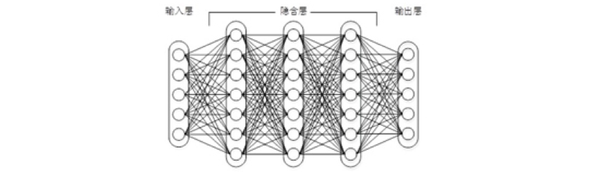
\includegraphics[width=\textwidth]{mlp}
  \caption{上下层神经元全部相连的神经网络——多层感知器}
  \label{fig:mlp}
\end{figure}

显然感知器的层数越多,其刻画现实的能力就越强,不过要让神经网络变深并不容易。
首先随着层数增加,\emph{优化函数越来越容易陷入局部最优解}, 并且这个“陷阱”越来越偏离真正的全局最优。
数据量不大时训练出的深层网络,性能还不如较浅层网络。其次\emph{“梯度消失”现象更加严重},
以sigmoid激活函数为例, 对于幅度为1的信号, 在BP反向传播梯度时,每传递一层,梯度衰减为原来的0.20,
这样层数一多,梯度指数衰减后低层的梯度几乎为0,
找不到合适的迭代方向。最后深层网络将产生海量的参数,
对训练算法和计算机硬件都要求很高.

上述问题都很难解决,所以九十年代, 大家都转而研究浅层学习模型,相继提出了支撑向量机(SVM,Support
Vector Machines)、 Boosting、最大熵方法(如LR,Logistic
Regression)等。这些模型的结构基本上可以看成带有一层隐层节点(如SVM、Boosting),或没有隐层节点(如LR),
此时神经网络的研究相对沉寂.
不过卷积神经网络(CNN)是一个特例, 它在层数增多的时候相对容易训练且效果很好,
所以在1998年提出后, 很快就被美国大多数银行用于支票等单据的手写数字识别.
CNN的易于训练的性质还没有在理论上找到明确的原因.

2006年,加拿大多伦多大学教授、机器学习领域的泰斗Geoffrey Hinton和
他的学生Ruslan Salakhutdinov在《科学》上发表了一篇文章\cite{hinton2006reducing},
开启了深度学习在学术界和工业界的新纪元。
他们利用预训练方法缓解了局部最优解问题, 将隐层数提升到了7.
所谓预训练就是在做有监督学习之前先做无监督学习, 用无监督学习出一些优异的特征
这样再做有监督学习可以得到更好的效果. Hinton使用了逐层优化的
多层限制玻尔兹曼机(Restricted Boltzmann machine, RBM),
又称作Deep Belif Network(DBN). 之后Vincent等\cite{vincent2008extracting}
提出了更好训练的Denoise autoencoder(dA)模型, 也可以做无监督的特征学习.

\section{卷积神经网络(CNN)}
1998年LeCun等\cite{lecun1998gradient}将CNN运用于手写数字识别, 取得了巨大
的成功, 下面结合手写数字数据集MINIST介绍CNN. \autoref{fig:cnn}
是一个典型的CNN网络, 它包括两个卷积层和一个全连接层.
\begin{figure}[htb]
  \centering
  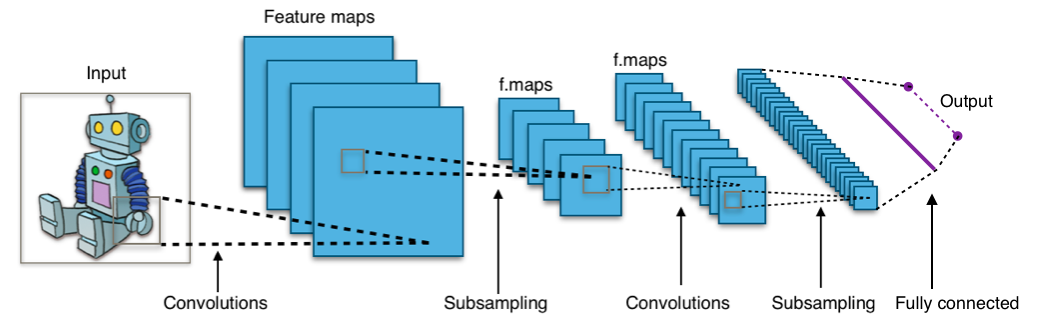
\includegraphics[width=.8\textwidth]{Typical_cnn}
  \caption{CNN结构}
  \label{fig:cnn}
\end{figure}

MNIST是一个入门级的计算机视觉数据集,它包含各种手写数字图片\\
{\centering
  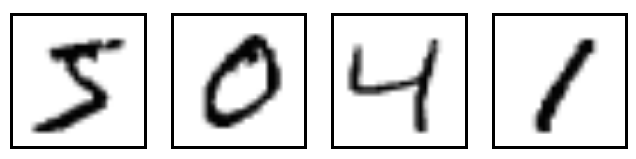
\includegraphics[width=.8\textwidth]{minist}

}
它也包含每一张图片对应的标签,告诉我们这个是数字几。
比如,上面这四张图片的标签分别是5,0,4,1。
我们要训练一个机器学习模型用于预测图片里面的数字.

\subsection{卷积}

首先介绍卷积, 直接给出一个具体的例子:假设你已经有
一个3x3的卷积核, 那么就可以用它提取5x5的样本所具有的特征.
如\autoref{fig:conv}所示, 我们对5x5的图像的每个3x3 的小块
图像区域都进行卷积运算, 结果变为3x3个卷积特征.
\begin{figure}[htb]
  \centering
  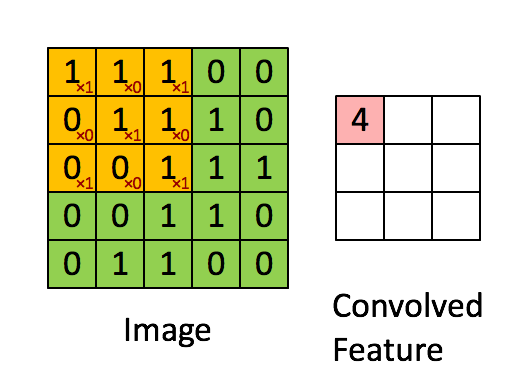
\includegraphics[width=.8\textwidth]{conv}
  \caption{对每个小块做卷积}
  \label{fig:conv}
\end{figure}

对于一个复杂的图片, 一种卷积核能提取的特征很有限, 需要
结合多种卷积核. CNN一个不同于以往方法之处就是没有人为
指定卷积核, 而是通过数据学习出来. CNN的一个卷积层如\autoref{fig:convlayer}
所示. 我们指定卷积核的个数\(k\), 然后作用于上一层的每一输入图片,
这样下一层的图片就更上一层的\(k\)倍.
\begin{figure}[htb]
  \centering
  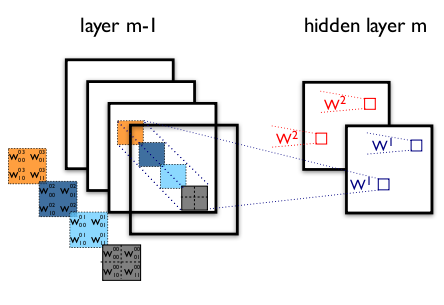
\includegraphics[width=.8\textwidth]{convlayer}
  \caption{CNN的一个卷积层}
  \label{fig:convlayer}
\end{figure}

\subsection{池化}
CNN的另一个重要概念是池化(Max-pooling).
它可以降采样, 加快运算速度, 又提供了某种
平移不变性. 池化很简单, 如2x2池化如\autoref{fig:maxpool}所示,
将4x4的图片降到2x2.
\begin{figure}[htb]
  \centering
  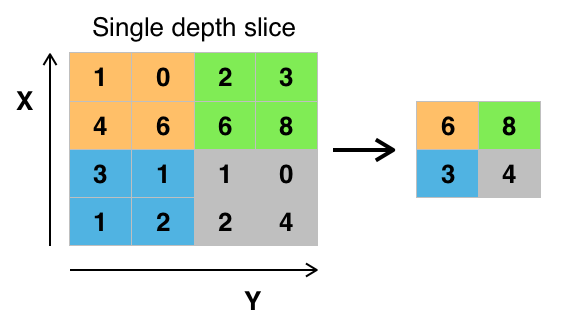
\includegraphics[width=.8\textwidth]{Max_pooling}
  \caption{最大池化}
  \label{fig:maxpool}
\end{figure}

\subsection{TensorFLow实现}
TensorFlow提供了卷积和池化的函数, 如果把每一层的输入\(x\)
看作一个4维矩阵(由于可能有RGB信息, 图片是三维矩阵,那么多张
图片就是4维), 即一个张量(tensor), 并且卷积核参数\(W\)
也是一个4维张量. 我们使用下面的函数计算卷积和池化.
\begin{lstlisting}
def conv2d(x, W):
  return tf.nn.conv2d(x, W, strides=[1, 1, 1, 1], padding='SAME')

def max_pool_2x2(x):
  return tf.nn.max_pool(x, ksize=[1, 2, 2, 1],
                        strides=[1, 2, 2, 1], padding='SAME')
\end{lstlisting}

由于MINIST的输入图片是\(28\times28\)的灰度图片, 所以初始化为
\(n\times28\times28\times1\)的张量. 设卷积在每个5x5的patch中算出32个特征
于是\(w\)是\(5\times5\times1\times32\).
\begin{lstlisting}
x_image = tf.reshape(x, [-1,28,28,1])
# 初始化第一个隐层的参数
W_conv1 = weight_variable([5, 5, 1, 32])
b_conv1 = bias_variable([32])
# 计算第一个隐层
h_conv1 = tf.nn.relu(conv2d(x_image, W_conv1) + b_conv1)
h_pool1 = max_pool_2x2(h_conv1)
\end{lstlisting}
第二个隐层类似, 只是取了64个特征. 经过两次池化,
图片尺寸减小到7x7,我们加入一个有1024个神经元的全连接层, 然后用
Softmax分类器即可. 这里还有一个防止过拟合的技巧:Dropout, 因为
全连接层有1024个神经元, 数量较多, 可以在每次训练时随机舍弃一些
神经元, 即dropout. 训练和预测代码如下, CNN在测试集上的准确率达到
了99.2\%.
\begin{lstlisting}
cross_entropy = -tf.reduce_sum(y_*tf.log(y_conv))
train_step = tf.train.AdamOptimizer(1e-4).minimize(cross_entropy)
correct_prediction = tf.equal(tf.argmax(y_conv,1), tf.argmax(y_,1))
accuracy = tf.reduce_mean(tf.cast(correct_prediction, "float"))
sess.run(tf.initialize_all_variables())
for i in range(20000):
  batch = mnist.train.next_batch(50)
  if i%100 == 0:
    train_accuracy = accuracy.eval(feed_dict={
        x:batch[0], y_: batch[1], keep_prob: 1.0})
    print "step %d, training accuracy %g"%(i, train_accuracy)
  train_step.run(feed_dict={x: batch[0], y_: batch[1], keep_prob: 0.5})

print "test accuracy %g"%accuracy.eval(feed_dict={
    x: mnist.test.images, y_: mnist.test.labels, keep_prob: 1.0})
\end{lstlisting}

\section{RBM和Autoencoder}
下面介绍Hinton在2006年提出的deep belief network(DBN). Hinton用DBN做
无监督学习的特征提取, 使用DBN后再用LR, SVM等分类器通常可以得到更好的
结果. DBN是逐层优化的限制玻尔兹曼机(RBM), 所以下面先介绍RBM.

RBM的想法是我们观测到的特征是有一些无法观测到的隐层特征决定的,
假定隐层变量互相独立, 且满足某种特定分布(一般取0-1的二项分布),
那么我们可以用这种结构, 模拟任何一种分布, 并通过极大似然估计的
方法确定出模型参数. 这样我们得到的隐层特征就是更本质的特征.
\begin{figure}[htb]
  \centering
  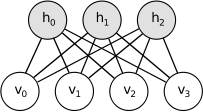
\includegraphics[width=.8\textwidth]{rbm}
  \caption{RBM是一个二部图: v是观测, h是隐层}
  \label{fig:rbm}
\end{figure}

\autoref{fig:rbm}的能量函数\(E(v,h)\)定义为:
\[
  E(v,h) = - b^Tv - c^Th - h^TWv
\]
一般情况下假设 \(v_j, h_i \in \{0,1\}\), 那么
可以推出下面两个条件概率:
\begin{align*}
  \P(h_i=1|v)& = \sigm(c_i + W_i v), \\
  \P(v_j=1|h)& = \sigm(b_j + W'_j h).
\end{align*}
下一步要得出参数的梯度, 这里需要用到Gibbs采样和Hinton提出的Contrastive
Divergence算法.
RBM模型具体的理论推导以及算法可以参考\cite{fischer2012introduction}.

RBM的TensorFlow实现也相对比较复杂, 不过
\url{http://deep-learning-tensorflow.readthedocs.io/en/stable/}
给出了包括RBM在内的很多模型的开源实现.

继DBN后, Bengio等\cite{bengio2007greedy}提出了一种类似的
特征提取深度网络: deep autoencoder(DAE). 它也是一种逐层优化的结构, 其中
最基础的一层如\autoref{fig:autoencoder}所示. 如果原始输入
是6维, 隐层是3个节点, 输出也是6个. 输入到隐层是encode, 隐层
到输出是decode.
\begin{figure}[htb]
  \centering
  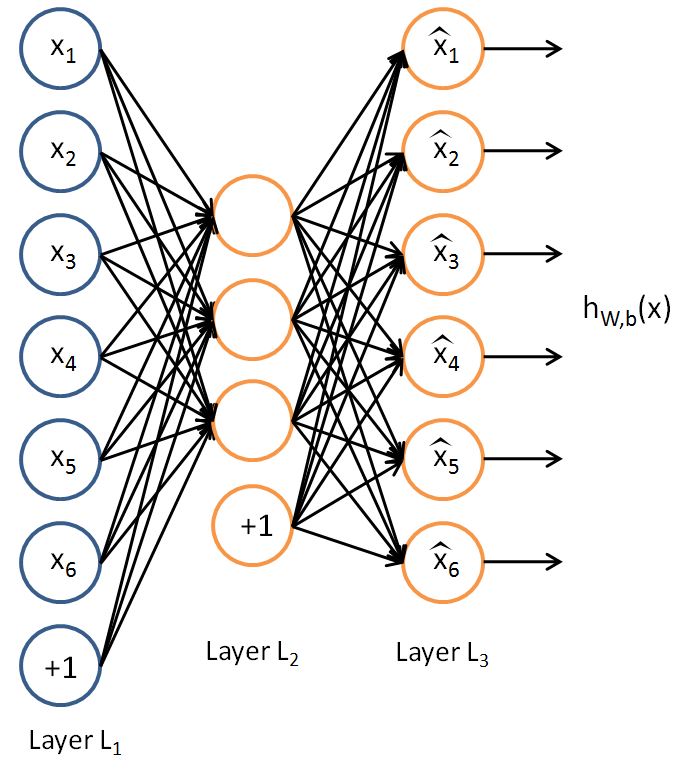
\includegraphics[width=.8\textwidth]{autoencoder}
  \caption{Autoencoder}
  \label{fig:autoencoder}
\end{figure}

最简单的情形, autoencoder将\( \mathbf{x} \in \mathbb{R}^d\)
映射到\(\mathbf{h} \in \mathbb{R}^p\)
\[
  \mathbf{h} = \sigma_1(\mathbf{Wx}+\mathbf{b})
\]
然后我们再从\(\mathbf{h}\)中重建\(mathbf{x}\)
\[
  \mathbf{x'} = \sigma_2(\mathbf{W'h}+\mathbf{b'})
\]
Autoencoder的目标就是极小化重建误差:
\[
  \mathcal{L}(\mathbf{x},\mathbf{x'})=
  \|\mathbf{x}-\mathbf{x'}\|^2=
  \|\mathbf{x}-\sigma_2(\mathbf{W'}(\sigma_1(\mathbf{Wx}+\mathbf{b}))+\mathbf{b'})\|^2
\]
对于一次优化后的结果, 我们可以去掉\(W', b'\), 继续将\(\mathbf{h}\)作为
下一层的输入优化新的一层. Deep autoencoder相对DBN计算量小, 在应用中它们
的表现互有胜负, \cite{cho2013boltzmann,deng2010binary}在图片识别和语音识别
领域对它们做了比较.

\section{LSTM和RNN}
未完成

\section{广告应用}
深度学习在很多方面取得的巨大成功, 比如图片识别领域, 现在ImageNet上识别率较高的
模型几乎没有不采用神经网络的. 不过在广告领域还没有看到公认的巨大成果, 百度宣称使用
DNN模型使得点击率预估准确率提升了20\%, 但是没有说清楚比较的基准是普通的
LR模型, 还是也是非线性的GBDT+FM.
目前也没有公司公开的自己用于广告的深度学习模型, 不过还是有些学术上的研究成果.

Zhang等\cite{zhang2016deep}提出了基于FM的Factorization-machine supported Neural
Network(FNN)和基于RBM, DAE的SNN两种模型改进CTR估计.

\printbibliography

\end{document}

